\documentclass{beamer}

\usepackage{multicol}
\usepackage[utf8]{inputenc}
\usepackage{minted}
\usepackage{amsfonts}
\usepackage{amsmath}
\usepackage{amsfonts,amsmath,amssymb}
\usepackage[none]{hyphenat}
\usepackage{fancyhdr}
\usepackage{graphicx}
\usepackage{float}
\usepackage{xcolor}
\usepackage{hyperref}
\usepackage{mdframed}
\usepackage{systeme}


\usetheme[progressbar=frametitle]{metropolis}
\setbeamertemplate{frame numbering}[fraction]
\useoutertheme{metropolis}
\useinnertheme{metropolis}
\usefonttheme{metropolis}
\setbeamercolor{background canvas}{bg = white}

\usecolortheme{beaver}

\title[Beamer]{iFood - Campaign Analysis}
\author{by Erik Davino Vincent}
\date{}

\begin{document}
\metroset{block = fill}

\begin{frame}
\titlepage
\end{frame}

\begin{frame}[c]{Summary}\vspace{0pt}
\begin{enumerate}
\item The userbase\\
\item Userbase segmentation\\
	\begin{enumerate}
	\item Behavior Segmentation\\
	\item Clustering\\
	\end{enumerate}
\item Prediction Model
\item Prediction Results
\item Final Considerations
\end{enumerate}
\end{frame}

\begin{frame}[c]{The user base}\vspace{0pt}

\only<1>{
\begin{columns}
	\begin{column}{0.5\textwidth}
\begin{table}[]
\begin{tabular}{|c|c|c|}
\hline
              & Year Birth  & Income        \\ \hline
\textbf{mean} & 1968.83 & 52061  \\ \hline
\textbf{std}  & 11.83   & 21810  \\ \hline
\textbf{min}  & 1920 & 1730   \\ \hline
\textbf{max}  & 1996 & 250000 \\ \hline
\end{tabular}
\end{table}
	\end{column}
	\begin{column}{0.5\textwidth}
		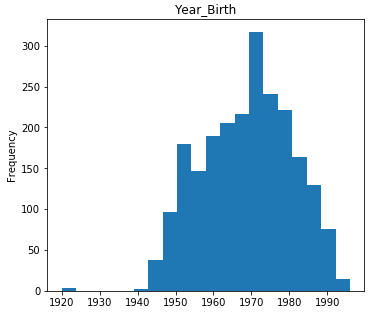
\includegraphics[scale=0.32]{Year_Birth.png}
		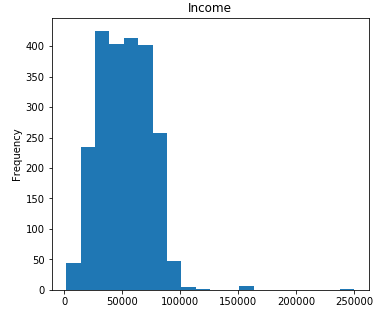
\includegraphics[scale=0.32]{Income.png}
	\end{column}
\end{columns}
}

\only<2>{
\begin{columns}
	\begin{column}{0.5\textwidth}
\begin{table}[]
\begin{tabular}{|c|c|c|}
\hline
              & Kid Home & Teen Home \\ \hline
\textbf{mean} & 0.444196 & 0.506250  \\ \hline
\textbf{std}  & 0.538398 & 0.544538  \\ \hline
\textbf{min}  & 0.000000 & 0.000000  \\ \hline
\textbf{max}  & 2.000000 & 2.000000  \\ \hline
\end{tabular}
\end{table}
	\end{column}
	\begin{column}{0.5\textwidth}
		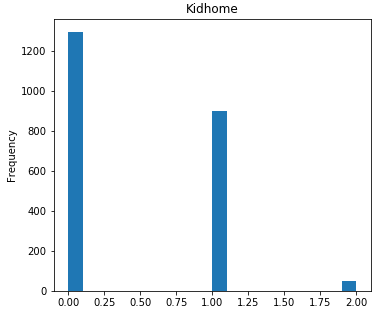
\includegraphics[scale=0.32]{Kid_Home.png}
		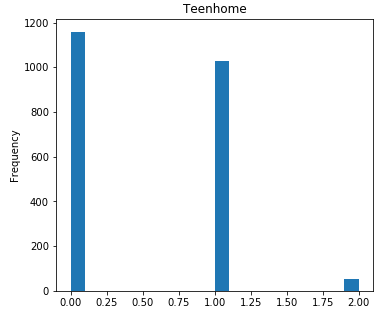
\includegraphics[scale=0.32]{Teen_Home.png}
	\end{column}
\end{columns}
}

\only<3>{
\begin{center}
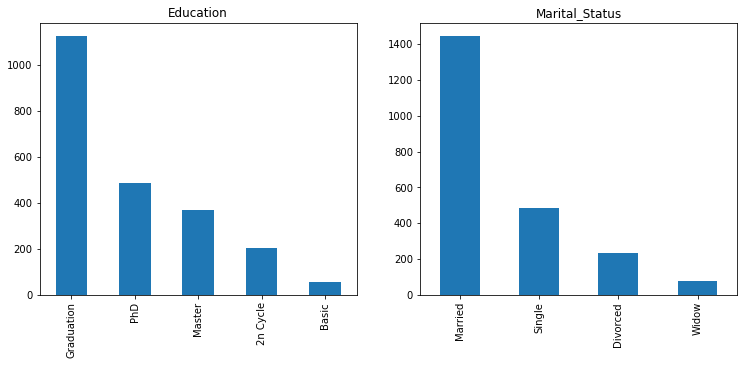
\includegraphics[scale=0.42]{Education_Marital_Status.png}
\end{center}
}

\only<4>{
\begin{itemize}
\item High level of education - graduation or higher
\item Most are married
\item At their mid to late fifties, but also a significant amount of younger and older users.
\item Almost half has at least one kid and/or teen at home
\item Medium income amount - middle class
\end{itemize}
}

\end{frame}

\begin{frame}[c]{Userbase Segmentation - Behavior}\vspace{0pt}

\only<1>{
\begin{itemize}
\item Most users don't buy large amounts - There is still a considerable amount of users who buy a lot.
\end{itemize}
\begin{center}
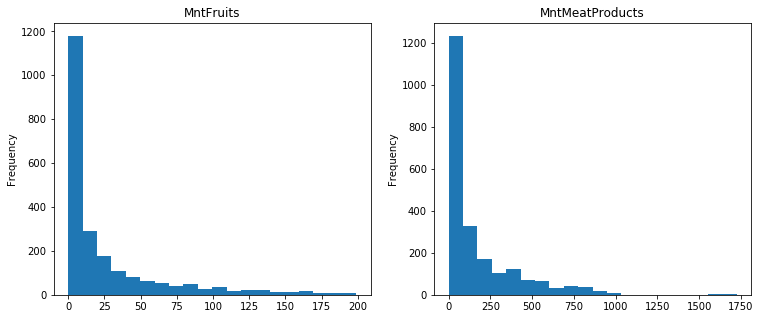
\includegraphics[scale=0.36]{Mnt_example.png}
\end{center}
}

\only<2>{
\begin{itemize}
\item Recency is uniformily distributed - There are as many users who come back often as there are users who don't
\item Most users don't visit the site very often
\end{itemize}
\begin{columns}
	\begin{column}{0.5\textwidth}
		\begin{center}
		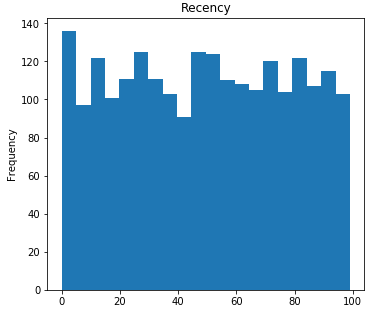
\includegraphics[scale=0.36]{Recency.png}
		\end{center}
	\end{column}
	\begin{column}{0.5\textwidth}
		\begin{center}
		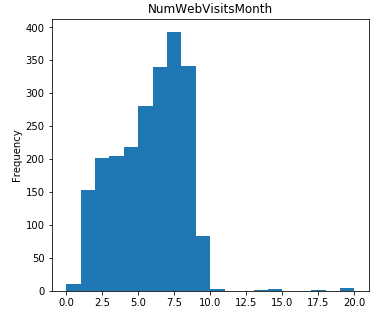
\includegraphics[scale=0.36]{numweb.png}
		\end{center}
	\end{column}
\end{columns}
}

\only<3>{
Preferred purchasing method
\begin{columns}
	\begin{column}{0.5\textwidth}
		\begin{center}
		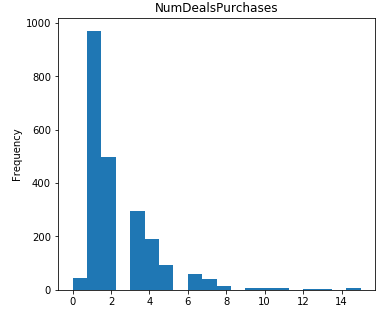
\includegraphics[scale=0.36]{numdealpur.png}
		\end{center}
	\end{column}
	\begin{column}{0.5\textwidth}
		\begin{center}
		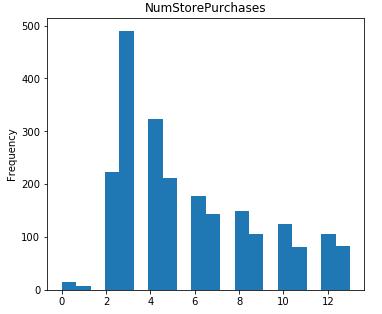
\includegraphics[scale=0.36]{numstorepur.png}
		\end{center}
	\end{column}
\end{columns}
}

\only<4>{
Preferred purchasing method
\begin{center}
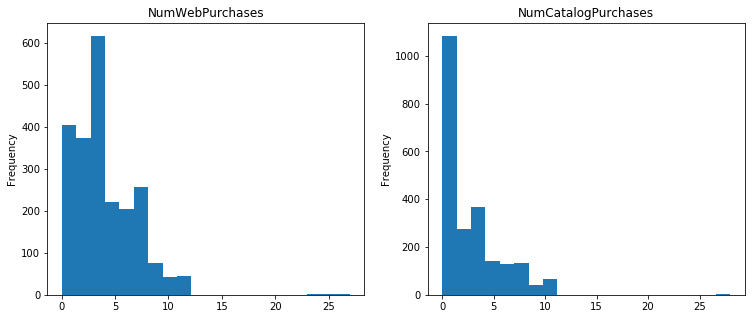
\includegraphics[scale=0.36]{numweb_numcatpur.png}
\end{center}
}

\only<5>{
Correlation:
\begin{itemize}
\item Positive correlation between having kids at home and lower income
\item Positive correlation between age and higher income
\item Positive correlation between having teenagers home and number of web purchases
\item Positive correlation between the amount of products bought
\item Positive correlation between number of web visits and number of deals purchases
\item Positive correlation between accepting different campaign offers, including the current one
\end{itemize}
}

\only<6>{
Based on the analysis of the data we can segment the users into the following categories:
}

\only<7>{
\textbf{A.}
\begin{itemize}
\item High income
\item Purchases a lot o products
\item More likely to purchase luxury products
\item Older and have no kids, but may have teenagers
\item Prefer store and catalog purchases
\end{itemize} 
}

\only<8>{
\textbf{B.}
\begin{itemize}
\item Low income - at the start of their careers or students
\item Don't buy a lot o products
\item A lot less likely to purchase luxury products
\item Younger and have no kids
\item Check the webservice more frequently
\end{itemize} 
}

\only<9>{
\textbf{C.}
\begin{itemize}
\item Low income
\item Don't buy a lot o products
\item A lot less likely to purchase luxury products
\item Younger - have kids and or teenagers at home
\item Don't use webservice very often
\end{itemize} 
}

\only<10>{
\textbf{D.}
\begin{itemize}
\item Medium income - majority of the userbase
\item Buy moderate amounts
\item More likely to use webservices and make deals purchases
\item Neither young nor old - likely have kids/teenagers at home
\item Use webservice more often
\end{itemize} 
}

\only<11>{
\textbf{E.}
\begin{itemize}
\item Trusty user base
\item Have taken offers brefore
\item Likely to take a new offer
\item Buy larger amounts
\item Medium to high income
\end{itemize} 
}

\end{frame}

\begin{frame}[c]{Userbase Segmentation - Clustering}\vspace{0pt}

\only<1>{
\begin{figure}
\begin{center}
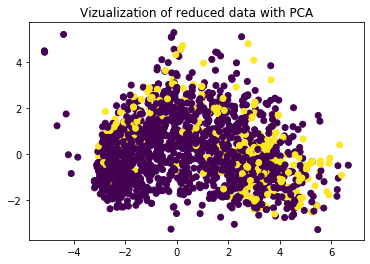
\includegraphics[scale=0.6]{pca_redc.png}
\end{center}
\caption{Legend: Yellow - Accepted Offer; Purple - Didn't Accept Offer}
\end{figure}
}

\only<2>{
\begin{figure}
\begin{center}
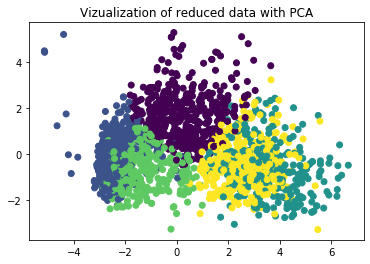
\includegraphics[scale=0.6]{pca_redc_groups.png}
\end{center}
\caption{Different groups found by k-means algorithm}
\end{figure}
}

\only<3>{
Based on the K-means generated groups, we can try and define the main characteristics of these groups as the following:
}

\only<4>{
\textbf{Group 1}
\begin{itemize}
\item Low income
\item More likely to make deals purchases
\item Buy smaller amounts
\item Youngest userbase - have children home
\item Lower recency
\item Make more webvisists but don't buy a lot through the web.
\end{itemize}
}

\only<5>{
\textbf{Group 2}
\begin{itemize}
\item Middle class
\item Buy larger amounts
\item Younger on average - have no kids or teenagers
\item Lower recency
\item More likely to give a positive response to the campaign offers, including the new one
\end{itemize}
}

\only<6>{
\textbf{Group 3}
\begin{itemize}
\item Middle class
\item Buy larger amounts
\item Older on average - have no kids
\item Prefer to make catalog purchases
\item High recency time
\item The most likely to give a positive response to the campaign offers, including the new one - 'loyal' userbase.
\end{itemize}
}

\only<7>{
\textbf{Group 4}
\begin{itemize}
\item Low to medium income
\item Buy smaller amounts
\item Spend a lot on meats and wines despite lower average income
\item Old group - have no kids but have teenagers
\item Makes web purchases the most - it's likely that their children do make them
\end{itemize}
}

\only<8>{
\textbf{Group 5}
\begin{itemize}
\item Lower income
\item The oldest group
\item Buy smaller amounts
\item Have high recency time
\item They have kids and/or teenagers at home
\item The least likely to take campaign offers
\end{itemize}
}

\end{frame}

\begin{frame}[c]{Prediction Model}\vspace{0pt}

\only<1>{
Machine Learning:
\begin{itemize}
\item Can make good predictions
\item Can be very fast
\item 'Learns' about the data by itself
\item Feature importance can be used to better understand data and the algorithm's predictions
\end{itemize}
}

\only<2>{
Results on training set:
\begin{table}[]
\begin{tabular}{c|cc|c|c|}
\cline{2-5}
                               & \multicolumn{1}{c|}{Precision} & Recall & f1-score & Support \\ \hline
\multicolumn{1}{|c|}{0}        & \multicolumn{1}{c|}{0.93}      & 0.99   & 0.96     & 1527    \\ \hline
\multicolumn{1}{|c|}{1}        & \multicolumn{1}{c|}{0.93}      & 0.55   & 0.69     & 265     \\ \hline
\multicolumn{1}{|c|}{Accuracy} &                                &        & 0.93     & 1792    \\ \hline
\multicolumn{1}{|c|}{Macro}    & \multicolumn{1}{c|}{0.93}      & 0.77   & 0.82     & 1792    \\ \hline
\multicolumn{1}{|c|}{Weighted} & \multicolumn{1}{c|}{0.93}      & 0.93   & 0.92     & 1792    \\ \hline
\end{tabular}
\end{table}
}

\only<3>{
Results on test set:
\begin{table}[]
\begin{tabular}{c|cc|c|c|}
\cline{2-5}
                               & \multicolumn{1}{c|}{Precision} & Recall & f1-score & Support \\ \hline
\multicolumn{1}{|c|}{0}        & \multicolumn{1}{c|}{0.90}      & 0.98   & 0.94     & 379     \\ \hline
\multicolumn{1}{|c|}{1}        & \multicolumn{1}{c|}{0.76}      & 0.42   & 0.54     & 69      \\ \hline
\multicolumn{1}{|c|}{Accuracy} &                                &        & 0.89     & 448     \\ \hline
\multicolumn{1}{|c|}{Macro}    & \multicolumn{1}{c|}{0.83}      & 0.70   & 0.74     & 448     \\ \hline
\multicolumn{1}{|c|}{Weighted} & \multicolumn{1}{c|}{0.88}      & 0.89   & 0.88     & 448     \\ \hline
\end{tabular}
\end{table}
}

\end{frame}

\begin{frame}[c]{Prediction Results}\vspace{0pt}

\only<1>{
Simulation Parameters:
\begin{itemize}
\item 448 users to make the offer or not
\item Campaign cost for each user: 3 MU
\item Campaign revenue for each user if the offer is accepted: 11 MU
\end{itemize}
}

\only<2>{
Simulation Results:
\begin{itemize}
\item Offer made to 50 users out of 448 MU
\item Estimated cost: 150 MU
\item Estimated revenue: 396 MU
\item Estimated profit: 246 MU
\item Gross profit margin ratio: 164\%
\item Campaign success rate: 72\%
\end{itemize}
}

\end{frame}

\begin{frame}[c]{Final Considerations}\vspace{0pt}

\only<1>{
Who accepted the campaign?
\begin{itemize}
\item Higher income on average
\item Lower recency
\item Smaller purchase amounts
\item More web and catalog purchases
\item Have accepted previous campaign offers
\end{itemize}
}

\only<2>{
Prediction model and results
\begin{itemize}
\item Easy to implement
\item Made good predictions
\item Can get better with more data
\item Provided a good profit margin with 72\% success rate on the test set
\end{itemize}
}

\end{frame}

\begin{frame}[standout]{The End}\vspace{0pt}
- Thank you for your time -
\end{frame}

















\end{document}
